\section{Thursday, March 13: Support Vector Machines}

Like Monday's class, today's class might at first seem like we are just randomly jumping to a new algorithm. But I hope that by the end of class, you are once again motivated to think of this instead as a new lens through which to study our important themes from the class. Today's theme is all about feature engineering in a really clever way, and what that gets us. SVMs also have some historical importance! 

\subsection{Motivation for SVMs}

To motivate today's class, we are going to be thinking about a picture that we haven't thought about since the day that we covered LDA. The picture is of two quantitative predictors $X_1$ and $X_2$, and a categorical response $y$ (shown by the colors). See Figure~\ref{fig_svm}.

Consider the left panel of Figure~\ref{fig_svm}. Our goal is to predict $Y$ using $X_1$ and $X_2$. In this case, the tasks looks almost unbelievably easy. The classes are linearly separable! A decision tree would actually do GREAT here, but pretend that we did not yet learn about decision trees. 

We learned during our LDA lecture that logistic regression, surprisingly, does quite badly in this perfectly separable case. If you try to fit a logistic regression in R to this data you will get warnings about convergence and ``fitted probabilities of 0 or 1" occurring. Logistic regression is all about modeling probabilities of $Y \mid X$, and there the estimates for certain regions all end up being $0$ or $1$, which makes the exact coefficients really uncertain. 

You can envision this problem a little bit in the middle panel of Figure~\ref{fig_svm}. All three lines perfectly separate the two classes, but they all have totally different slopes. How do we know which line to choose?

LDA and QDA chose between these different lines by making a very strong assumption. They assume that $X \mid Y$ is Gaussian. See the right panel of Figure~\ref{fig_svm}. Then, you can draw estimated Gaussian contour lines for each class. The decision boundary chosen by LDA or QDA has to do with when these contours are set equal to one another: when is the red class or the blue class more likely, given X, based on the estimated Gaussian densities?  

\begin{figure}
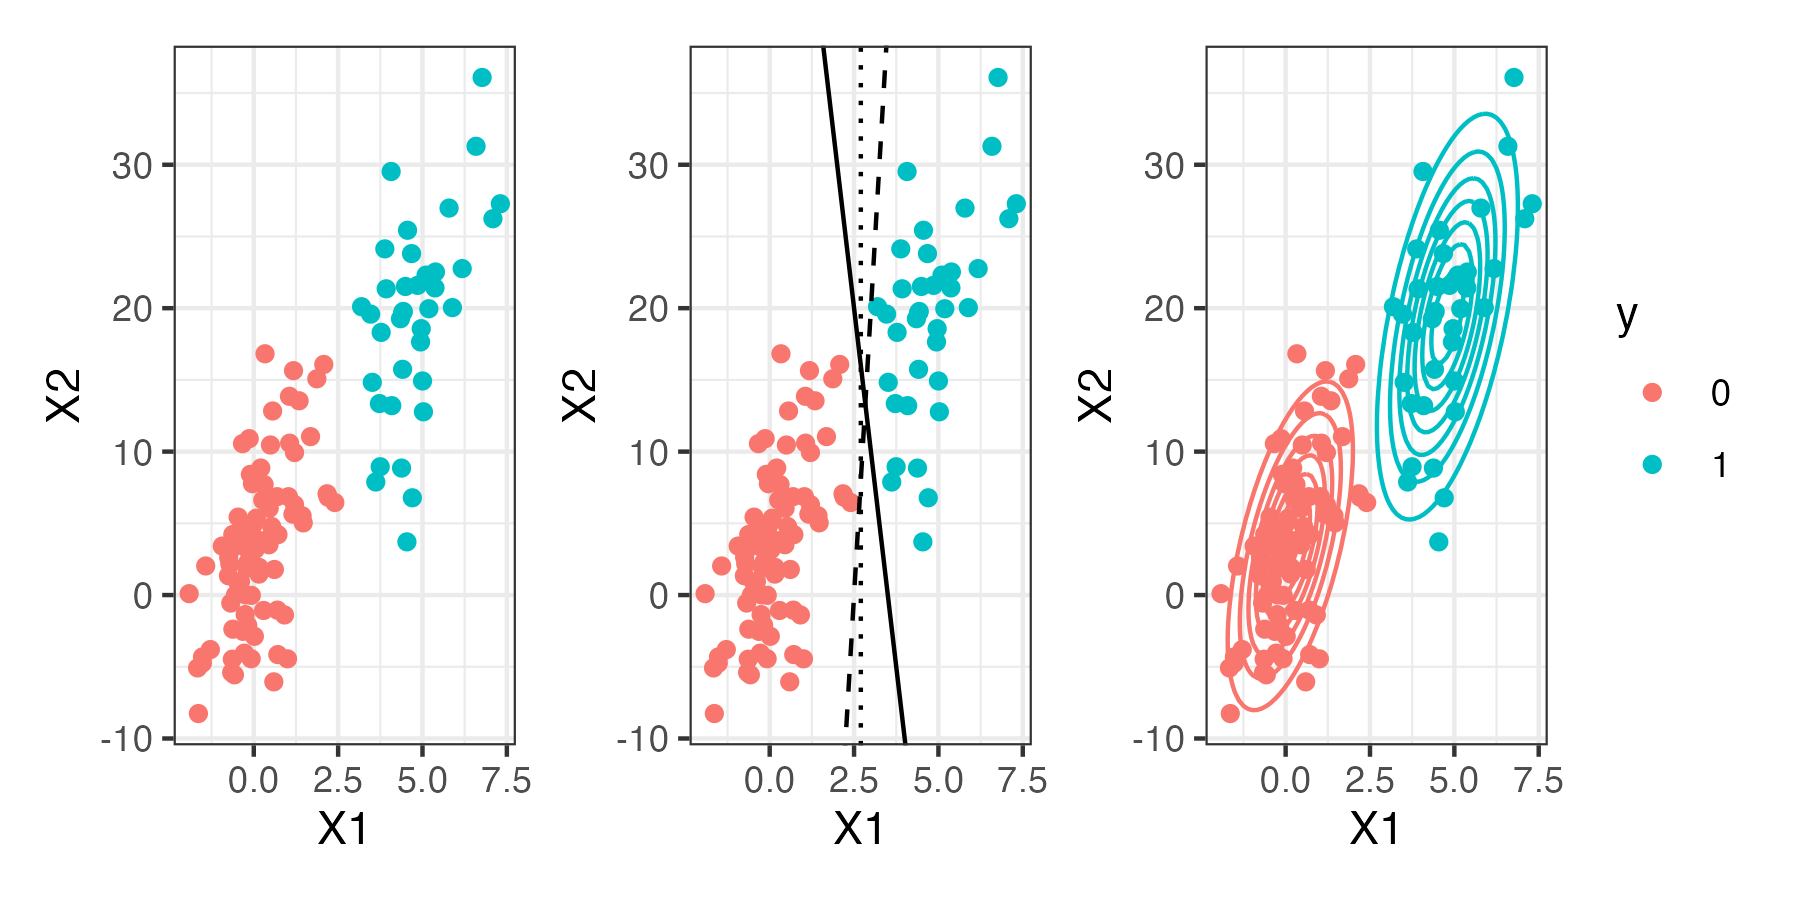
\includegraphics[width=\textwidth]{442_lecs/svm_raw.png}
\caption{A figure to motivate SVMs, and their differences with logistic regression, LDA, or QDA.}
\label{fig_svm}
\end{figure}

What if we want a way to pick between all of the lines in the center panel of Figure~\ref{fig_svm}? And we want a way that does not make a Gaussian assumption?  This is the idea of the maximum margin classifier, which Greta will tell us about in her presentation, and which is summarized in Figure~\ref{fig_svm2}, which is taken from ISL. The idea is quite simple: let's pick between all of the possible separating lines by choosing the one that is as far as possible from all of the training observations. 

\begin{figure}
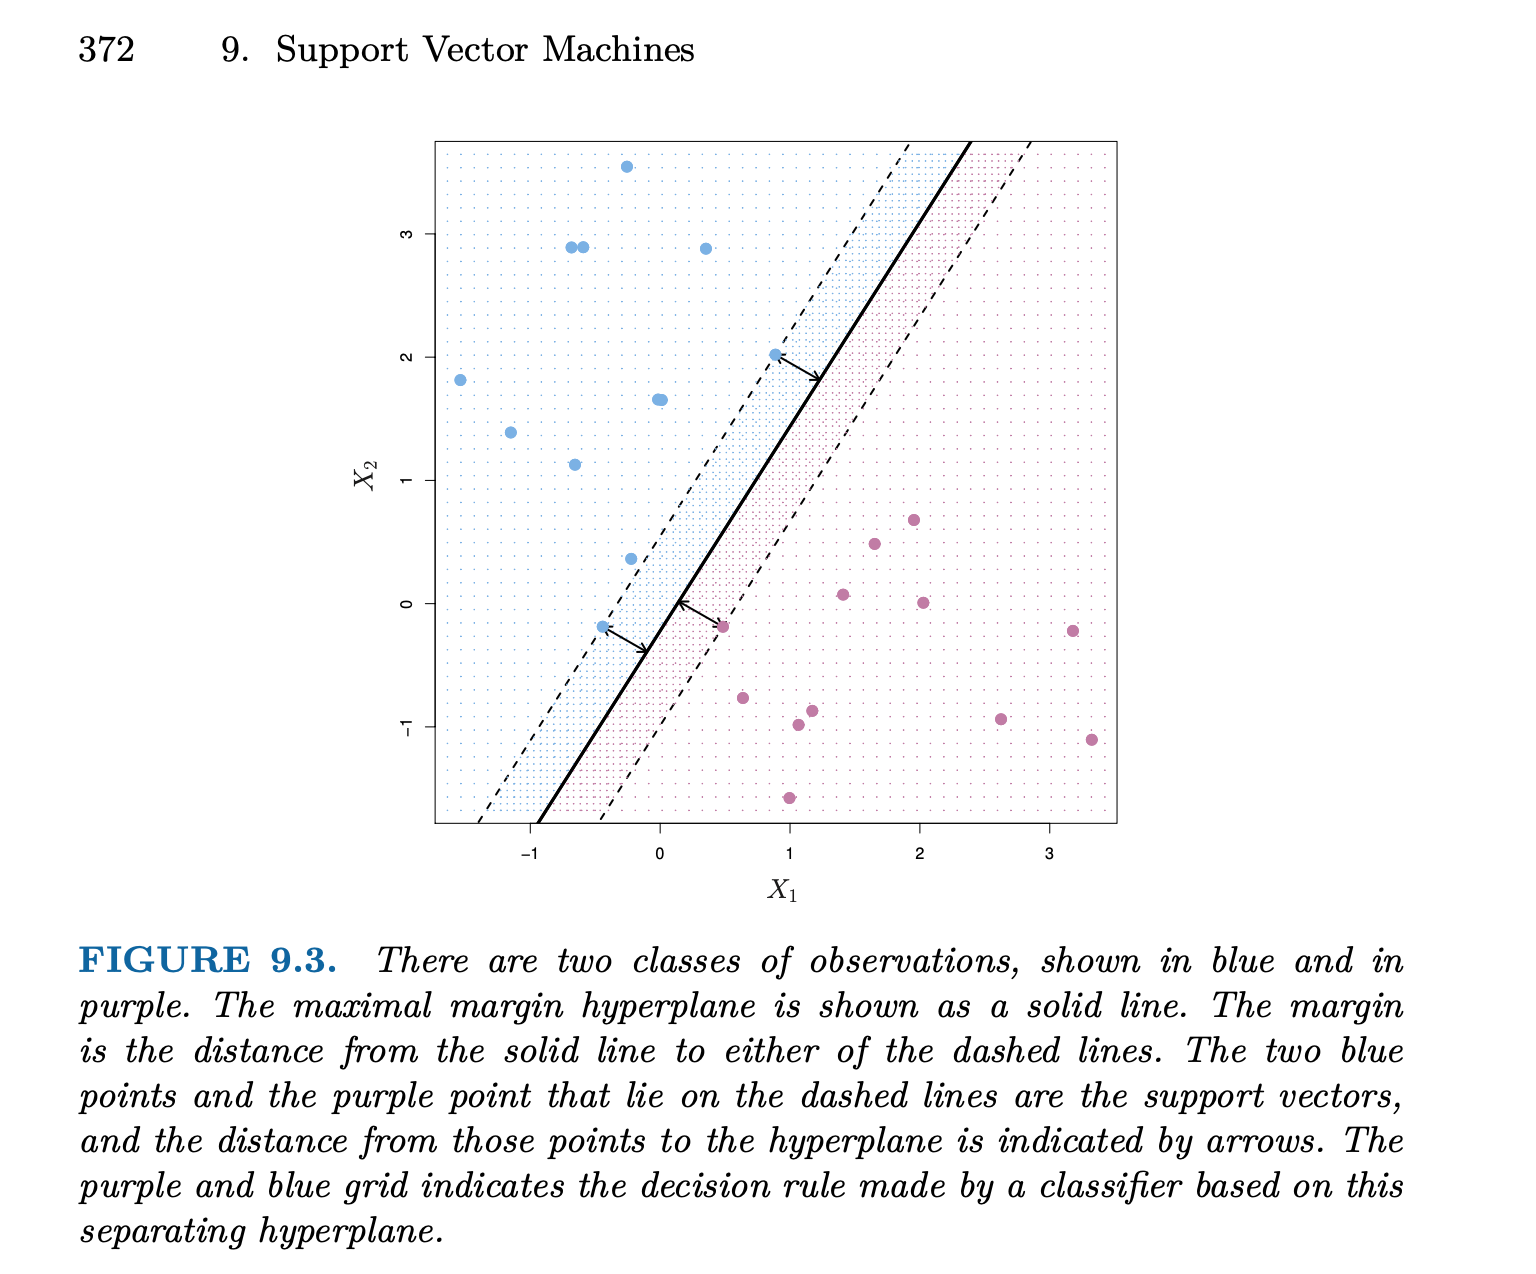
\includegraphics[width=0.8\textwidth]{442_lecs/svm.png}
\caption{The maximum margin classifier picks the line that is far as possible from all observations.}
\label{fig_svm2}
\end{figure}

\subsection{Maximum margin classifier using constrained optimization}

How do we actually fit the line in Figure~\ref{fig_svm2}? There is some math that relates to how we actually draw these lines onto plots. Also, note that we could have more than $2$ $X$ variables, and then we would be using a plane and not a line to separate our classes. 

In general, we will write our linear boundary as the line:
$$
\beta_0 + \beta_1 X_1 + \ldots + \beta_p X_p = 0. 
$$
The idea is to pick a line so that $\beta_0 + \beta_1 X_1 + \ldots + \beta_p X_p < 0$ whenever $y=-1$ and $\beta_0 + \beta_1 X_1 + \ldots + \beta_p X_p > 0$ whenever $y=1$. For today, we are doing binary classification and we are writing our two classes as $-1$ and $1$, for simplicity. 

Any of the lines in the center panel of Figure~\ref{fig_svm} actually have this property. So now the idea is to do even better. Let's both have it be the case that $\beta_0 + \beta_1 X_1 + \ldots + \beta_p X_p < 0$ whenever $y=-1$ and $\beta_0 + \beta_1 X_1 + \ldots + \beta_p X_p > 0$ whenever $y=1$, but also have it be the case that $\beta_0 + \beta_1 X_1 + \ldots + \beta_p X_p$ is basically never TOO close to $0$. Because when it is near $0$, it means that points are close to the line and we have uncertainty. 

%So, the maximum margin classifier says:


\subsection{From maximum margin classifier to support vector machines}



\subsection{Optimization}


\subsection{The kernel trick}


\subsection{What do we think about SVMs?}







